\documentclass[11pt,a4paper]{scrartcl}

\usepackage{../manostilius_lt}

\title{Daugianarių daugyba}
\author{Andrius Berniukevičius}

\begin{document}

\maketitle

\section{Skaičiaus ir sumos sandauga}

Pradėkime nuo žinomos aritmetikos taisyklės. Jei skaičių dauginame iš sumos, galime jį padauginti iš kiekvieno sumos dėmens ir gautas sandaugas sudėti.

\begin{property}[Skaičiaus ir sumos sandauga]
Bet kuriems skaičiams $a$, $b$ ir $c$ galioja lygybė:
\[
a(b+c)=ab+ac.
\]
\end{property}

Kodėl taip galima daryti? Sumą $b+c$ sudaro dvi dalys: $b$ ir $c$. Dauginant iš $a$, abi šios dalys padidinamos tuo pačiu $a$ kartų, todėl galime jas dauginti atskirai ir rezultatus sudėti.

\begin{example}
Apskaičiuokime:
\[
6(8+3).
\]
\textbf{Sprendimas}\\
Skaičių $6$ padauginame iš kiekvieno sumos dėmens:
\[
6(8+3)=6\cdot8+6\cdot3=48+18=66.
\]
Patikriname: $6(8+3)=6\cdot11=66$.
\textbf{Atsakymas:} $66$.
\end{example}

Tokia pati taisyklė galioja ir tada, kai vienas iš sumos dėmenų yra neigiamas:
\[
a(b-c)=a\bigl(b+(-c)\bigr)=ab+a(-c)=ab-ac.
\]

\section{Vienanario daugyba iš daugianario}

Daugianaris yra vienanarių algebrinė suma. Todėl daugindami vienanarį iš daugianario, taikome skaičiaus ir sumos sandaugos taisyklę kiekvienam daugianario nariui.

\begin{property}[Vienanario ir daugianario sandauga]
Norėdami padauginti vienanarį iš daugianario, vienanarį dauginame iš kiekvieno daugianario nario ir gautas sandaugas sudedame:
\[
k(a+b+c)=ka+kb+kc.
\]
\end{property}

\begin{proof}
Daugianarį $a+b+c$ galime suprasti kaip sumą $(a+b)+c$. Tuomet taikome skaičiaus ir sumos sandaugos taisyklę du kartus:
\[
k(a+b+c)=k\bigl((a+b)+c\bigr)=k(a+b)+kc.
\]
Dar kartą pritaikę tą pačią taisyklę gauname:
\[
k(a+b)+kc=ka+kb+kc.
\]
Vadinasi, vienanarį galima dauginti iš kiekvieno daugianario nario atskirai.
\end{proof}

\begin{example}
Supaprastinkite reiškinį:
\[
3x(2x^2-5x+4).
\]
\textbf{Sprendimas}\\
Vienanarį $3x$ dauginame iš kiekvieno daugianario nario:
\[
3x(2x^2-5x+4)=3x\cdot2x^2+3x\cdot(-5x)+3x\cdot4.
\]
Atliekame vienanarių daugybą:
\[
3x(2x^2-5x+4)=6x^3-15x^2+12x.
\]
\textbf{Atsakymas:} $6x^3-15x^2+12x$.
\end{example}

\begin{example}
Supaprastinkite reiškinį:
\[
-2a^2(3a^3-a+5).
\]
\textbf{Sprendimas}\\
\[
\begin{aligned}
-2a^2(3a^3-a+5)
&=(-2a^2)\cdot3a^3+(-2a^2)\cdot(-a)+(-2a^2)\cdot5 \\
&=-6a^5+2a^3-10a^2.
\end{aligned}
\]
\textbf{Atsakymas:} $-6a^5+2a^3-10a^2$.
\end{example}

\section{Dviejų dvinarių daugyba}

Padauginkime du dvinarius $(a+b)$ ir $(c+d)$. Pirmąjį dvinario dėmenį $c$ ir antrąjį dėmenį $d$ dauginame iš viso daugianario $(a+b)$:

\begin{property}[Dviejų dvinarių sandauga]
\[
(a+b)(c+d)=ac+ad+bc+bd.
\]
\end{property}

\begin{proof}
Pirmiausia antrąjį skliaustą suprantame kaip sumą ir taikome skaičiaus bei sumos sandaugos taisyklę:
\[
(a+b)(c+d)=(a+b)c+(a+b)d.
\]
Tuomet atskliaudžiame abu gautus reiškinius:
\[
(a+b)c+(a+b)d=ac+bc+ad+bd.
\]
Sukeitę vidurinių dėmenų tvarką gauname:
\[
(a+b)(c+d)=ac+ad+bc+bd.
\]
\end{proof}

Geometriškai šią formulę galime paaiškinti stačiakampio plotu. Nubrėžkime stačiakampį, kurio ilgis yra $a+b$, o plotis -- $c+d$:
\begin{center}
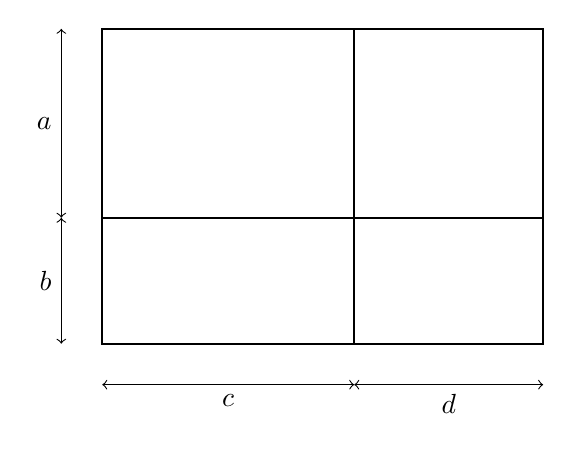
\begin{tikzpicture}[x=0.8cm,y=0.8cm]
	\draw[thick] (0,0) rectangle (7,5);
	\draw[thick] (4,0) -- (4,5);
	\draw[thick] (0,2) -- (7,2);
	\draw[<->] (0,-0.65) -- node[below] {$c$} (4,-0.65);
	\draw[<->] (4,-0.65) -- node[below] {$d$} (7,-0.65);
	\draw[<->] (-0.65,2) -- node[left] {$b$} (-0.65,0);
	\draw[<->] (-0.65,5) -- node[left] {$a$} (-0.65,2);
\end{tikzpicture}
\end{center}
Didžiojo stačiakampio plotas yra jo kraštinių sandauga:
\[
(a+b)(c+d).
\]
Tą patį stačiakampį galime laikyti sudarytu iš keturių mažesnių stačiakampių:
\begin{center}
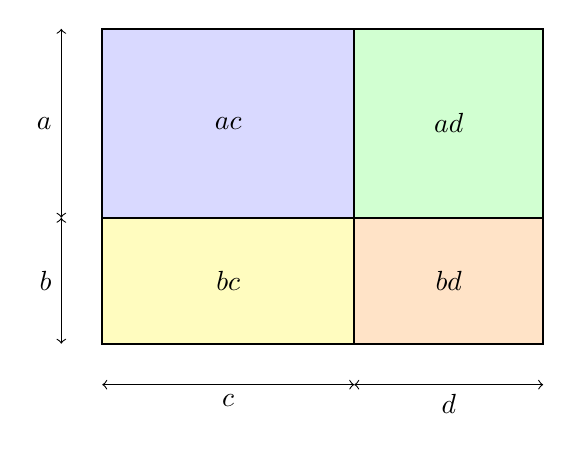
\begin{tikzpicture}[x=0.8cm,y=0.8cm]
	\fill[blue!15] (0,2) rectangle (4,5);
	\fill[green!18] (4,2) rectangle (7,5);
	\fill[yellow!25] (0,0) rectangle (4,2);
	\fill[orange!22] (4,0) rectangle (7,2);
	\draw[thick] (0,0) rectangle (7,5);
	\draw[thick] (4,0) -- (4,5);
	\draw[thick] (0,2) -- (7,2);
	\node at (2,3.5) {$ac$};
	\node at (5.5,3.5) {$ad$};
	\node at (2,1) {$bc$};
	\node at (5.5,1) {$bd$};
	\draw[<->] (0,-0.65) -- node[below] {$c$} (4,-0.65);
	\draw[<->] (4,-0.65) -- node[below] {$d$} (7,-0.65);
	\draw[<->] (-0.65,2) -- node[left] {$b$} (-0.65,0);
	\draw[<->] (-0.65,5) -- node[left] {$a$} (-0.65,2);
\end{tikzpicture}
\end{center}
Jų plotų suma yra $ac+ad+bc+bd$. Kadangi abiem būdais apskaičiuojame to paties didžiojo stačiakampio plotą, gauname:
\[
(a+b)(c+d)=ac+ad+bc+bd.
\]
\textbf{Išvada:} kiekvieną pirmojo daugianario narį dauginame iš kiekvieno antrojo daugianario nario. Šiuo atveju gauname keturias sandaugas.

\begin{example}
Supaprastinkite reiškinį:
\[
(x+3)(x+2).
\]
\textbf{Sprendimas}\\
Kiekvieną pirmojo skliausto narį dauginame iš kiekvieno antrojo skliausto nario:
\[
\begin{aligned}
(x+3)(x+2)
&=x\cdot x+x\cdot2+3\cdot x+3\cdot2 \\
&=x^2+2x+3x+6 \\
&=x^2+5x+6.
\end{aligned}
\]
\textbf{Atsakymas:} $x^2+5x+6$.
\end{example}

\section{Daugianario daugyba iš daugianario}

\begin{property}[Daugianarių daugyba]
Norėdami padauginti du daugianarius, kiekvieną pirmojo daugianario narį dauginame iš kiekvieno antrojo daugianario nario. Gautas sandaugas užrašome kaip algebrinę sumą ir sutraukiame panašiuosius vienanarius.
\end{property}

\begin{example}
Supaprastinkite reiškinį:
\[
(2x-1)(x^2+3x-4).
\]
\textbf{Sprendimas}\\
Pirmiausia daugianarį $x^2+3x-4$ dauginame iš $2x$, o paskui iš $-1$:
\[
\begin{aligned}
(2x-1)(x^2+3x-4)
&=2x(x^2+3x-4)-1(x^2+3x-4) \\
&=2x^3+6x^2-8x-x^2-3x+4 \\
&=2x^3+5x^2-11x+4.
\end{aligned}
\]
\textbf{Atsakymas:} $2x^3+5x^2-11x+4$.
\end{example}

\section{Uždaviniai}

\begin{problem}
Atskliauskite.
\begin{tasks}[label={(\arabic*)}, label-offset=0.9em](2)
	\task $4x(3x^2-2x+5)$
	\task $-3a^2(2a^3+a-4)$
	\task $5m^2(m^3-2m+1)$
	\task $-2p(4p^2-p-3)$
	\task $7ab(2a-b+3)$
	\task $-4x^2y(xy-2x+y)$
\end{tasks}
\end{problem}

\begin{problem}
Padauginkite dvinarius ir sutraukite panašiuosius vienanarius.
\begin{tasks}[label={(\arabic*)}, label-offset=0.9em](2)
	\task $(x+4)(x+2)$
	\task $(a-5)(a+3)$
	\task $(2m+1)(m-4)$
	\task $(3p-2)(p+5)$
	\task $(x-6)(2x-1)$
	\task $(4a+b)(a-2b)$
\end{tasks}
\end{problem}

\begin{problem}
Padauginkite daugianarius ir sutraukite panašiuosius vienanarius.
\begin{tasks}[label={(\arabic*)}, label-offset=0.9em](2)
	\task $(x+2)(x^2-x+3)$
	\task $(2a-3)(a^2+2a-1)$
	\task $(m-4)(m^2+3m+2)$
	\task $(3x+1)(x^2-2x+4)$
\end{tasks}
\end{problem}

\newpage
\answerssection

\begin{problem} \phantom{text}
\begin{tasks}[label={(\arabic*)}, label-offset=0.9em](2)
	\task $12x^3-8x^2+20x$;
	\task $-6a^5-3a^3+12a^2$;
	\task $5m^5-10m^3+5m^2$;
	\task $-8p^3+2p^2+6p$;
	\task $14a^2b-7ab^2+21ab$;
	\task $-4x^3y^2+8x^3y-4x^2y^2$.
\end{tasks}
\end{problem}

\begin{problem} \phantom{text}
\begin{tasks}[label={(\arabic*)}, label-offset=0.9em](2)
	\task $x^2+6x+8$;
	\task $a^2-2a-15$;
	\task $2m^2-7m-4$;
	\task $3p^2+13p-10$;
	\task $2x^2-13x+6$;
	\task $4a^2-7ab-2b^2$.
\end{tasks}
\end{problem}

\begin{problem} \phantom{text}
\begin{tasks}[label={(\arabic*)}, label-offset=0.9em](2)
	\task $x^3+x^2+x+6$;
	\task $2a^3+a^2-7a+3$;
	\task $m^3-m^2-10m-8$;
	\task $3x^3-5x^2+10x+4$.
\end{tasks}
\end{problem}

\end{document}
